\section{System design}
(recommended size: 1.5 pages)

\subsection{System overview}
The distributed system we designed consists of several server nodes and possibly many client nodes. Each client node represents a single player in the virtual world and connects to a single server. All servers contain the current state of the virtual world and they inform each other of game updates to keep the game states of the servers consistent. In this section we will provide more details on the design of the system by describing what happens within the system in the possible scenarios. The scenarios we will describe next are: connecting and disconnecting a client from the system, performing actions selected by a client and handling crashes of a server or client node.

\subsubsection*{(Dis)connecting clients}
The process of clients connecting to the server is visualized in Figure \ref{connect_diagram}. Every client node has a list of IP addresses of the game servers. When a new client wants to enter the game, it first randomly selects a server from this list and tries to connect with it (1). When the connection succeeds, the server first informs all other servers of the new client (2) and then it sends the current game state to the client as well as the identifier of the client (3). After the client receives this message it can start performing actions.

When the connection to a server cannot be established, the client simply selects another server from the list and tries again until one of the servers responds. So, in this way the process of connecting a client is fault-tolerant and is also scalable as all clients randomly select one of this servers which makes the expected load on each server equal.

Disconnecting a client works roughly in the same way. The client that wants to quit the game sends a message to the server it is connected to. Then this server informs the other servers of the client leaving the game and sends a confirmation to the client. Finally, upon receiving this confirmation the client shuts down the application.

\begin{figure}[h!]
  \centering
    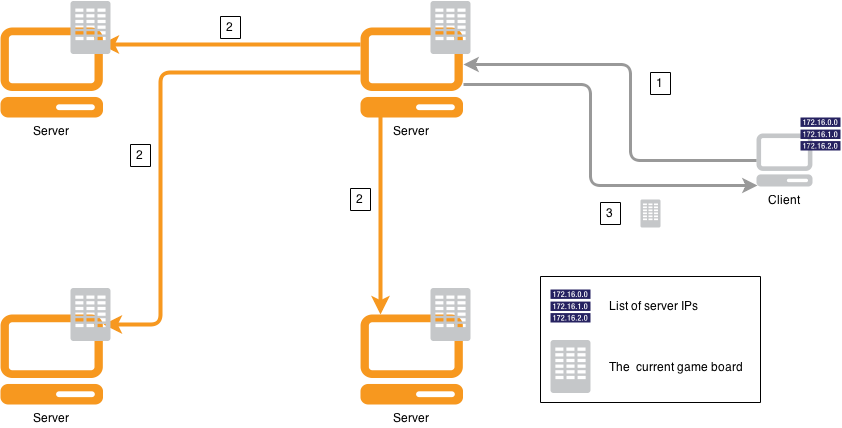
\includegraphics[width=\textwidth]{diagrams/connecting-client}
    
  \caption{A client connecting to a server}
  \label{connect_diagram}
\end{figure}

\subsubsection*{Clients performing actions}
This process of clients performing actions is visualized in Figure \ref{update_diagram}. When a client wants to perform an action, it sends a request for this action to the server it is connected to (1). Then the server first checks whether this action is valid and can be performed (to avoid clients spoofing requests). When the action is valid, the server will send a request for the action to all the other game servers (2). When the other servers agree on this action, they will send an acknowledgment back to the server (3). When the server receives an acknowledgment from all other servers, it knows the action can be performed and informs all other servers that the action has been executed (4). Finally, all servers send the update of the game state to all the connected clients (5).

This process of sending requests and acknowledgments it necessary to keep the game state consistent across all servers and therefore also all clients. Moreover, this process is also resilient against lost messages. When the client request (1) is lost, the action will simply not be performed. The same holds when one or more of the server requests (2) or acknowledgments (3) get lost. When one of the messages sent in step (4) gets lost, the action will still be performed, making the game state in the server to which the message was send (as well as its clients) inconsistent with the other servers. However, this inconsistency is only temporary as the next action of the same client will repair the missed update. This is the case because for instance the requests for a move do not contain the direction of the move, but instead the position on the grid to which the player wants to move.

\begin{figure}[h!]
  \centering
    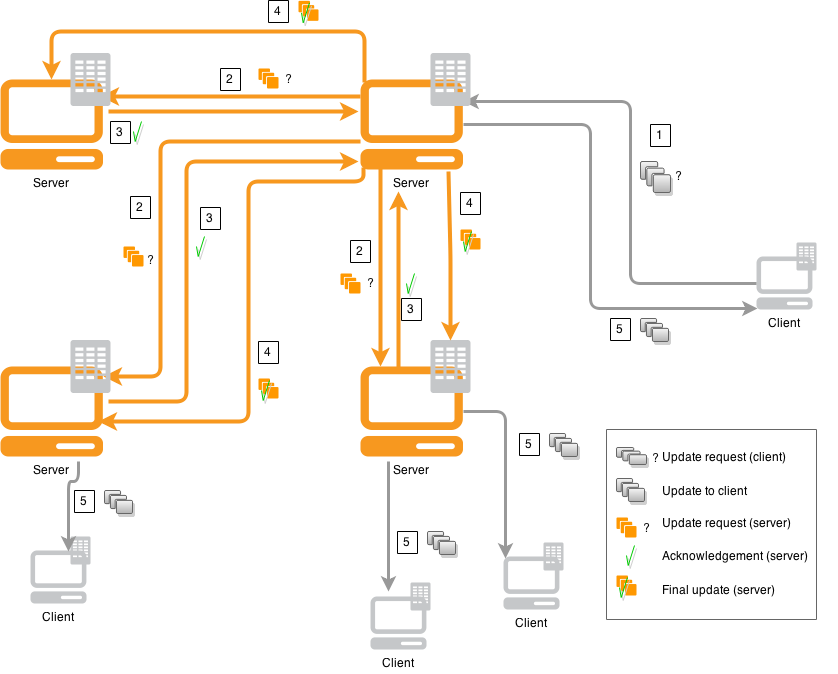
\includegraphics[width=\textwidth]{diagrams/game-update}
    
  \caption{A client sending an update to a server}
  \label{update_diagram}
\end{figure}

\subsubsection*{Client and server crashes}
The final scenario that we discuss in this chapter is the crash of a server or client node. To know when a certain server has crashed, the servers send heartbeat messages to each other. When a server has missed two consecutive heartbeat messages of a certain server it assumes that that server has crashed and it will stop sending messages to it. When this server comes back online, it will send a message to all other servers to let them know it is available again. Then one of the servers will send the current game state to the `new' server so it can start participating in the system again. 

Besides the heartbeat messages sent to other servers, the servers also send heartbeat messages to their clients to check if they are still connected. When a client misses two consecutive messages, it will be considered offline and will be removed from the game. When this client comes back online it can simply try to connect to one of the server as described above.

Finally, when a server misses two consecutive heartbeat messages from its client, the client assumes it has crashed. Then this client will pick another server from its lists of servers and try to connect to it so it can resume the game.

\subsection{Additional System Features}
(optional): Describe each additional feature of your system, one sub-section per feature
 